\begin{figure}[thb]
  \centering
  \begin{minipage}[b]{0.49\linewidth}
      \center
      \centerline{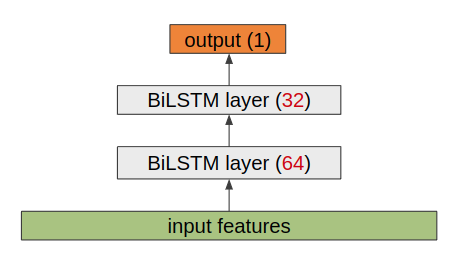
\includegraphics[width=5cm]{./Chapitre5/figures/biLSTM2.png}}
  \end{minipage}
  \begin{minipage}[b]{0.49\linewidth}
      \center
      \centerline{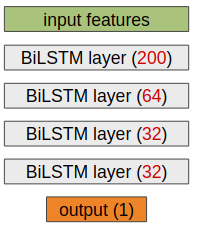
\includegraphics[width=5cm]{./Chapitre5/figures/biLSTM4.png}}
  \end{minipage}
    \caption{Schéma de la configuration des systèmes neuronaux appelés biLSTM-2 (à gauche) et biLSTM-4 (à droite). Le nombre de neurone est indiqué en rouge sur chaque couche. Comme il s'agit de réseaux bidirectionnels, il faut multiplier par deux le nombre de neurones pour avoir le nombre de paramètres réels.}
    \label{fig:biLSTM}
\end{figure}
